\subsection{Registration}
\paragraph{Purpose}
	Visitors can register to myTaxiService through the web or mobile application. They can register either as a passenger or as a taxi driver.\\
	In both cases, this operation requires the visitor to fill a registration form with personal data and accept myTaxiService terms and conditions, including personal data policies, according to local law. In case of registration as a taxi driver, the system requires the visitor more info, including proof of the possession of a valid taxi driver license.\\
	If any of the previous requirements are not met or any input is invalid, the registration fails and the system asks the visitor to repeat the process. Otherwise, a verification email is sent to the provided email address: from that email the visitor can confirm his new account and successfully end the registration process.

\paragraph{Scenarios}
	\begin{enumerate}
		\item Alex is a student. He has heard about myTaxiService and, finding it an easy way to travel, wants to subscribe to it.\\
		Therefore, he access to the homepage of the web application, clicks "Register", then chooses "Passenger". He fulfills the form, accepts the terms and conditions, and clicks "Confirm". However, the system cannot verify Alex's info because the confirmation password does not match with the first one. It therefore asks Alex to write it again. This time Alex fills the form correctly, then clicks "Confirm". The system verifies his info, then sends Alex a verification email to the submitted email address. Alex checks his mailbox, opens the new mail and clicks on the link inside it, redirecting him back to the web application of myTaxiService. The system informs him that the registration has successfully ended. He can now log in as a passenger user.
			
		\item Bob is a taxi driver. His company recommends him to subscribe to myTaxiService, in order to make his work easier and improve the taxi service.\\
		Therefore, he downloads and installs the mobile app of myTaxiService on his mobile phone, then opens it. He taps "Register", then chooses "Taxi Driver". He inputs all the required data, including his driver license ID, accepts the terms and conditions and confirms. The system verifies the submitted info and sends Bob a confirmation email. Bob checks his mailbox, opens the new mail and taps on the link inside. The system informs him that the registration has successfully ended. He can now log in as a taxi driver user.
	\end{enumerate}

\paragraph{Diagrams}
	\begin{center}
		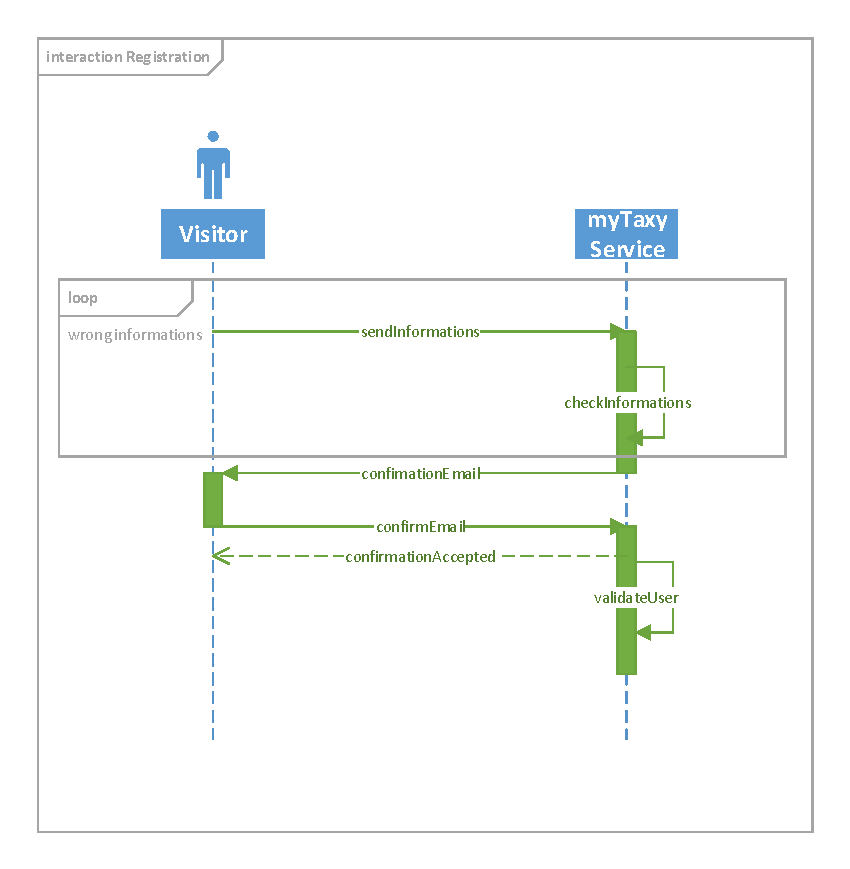
\includegraphics[width=\textwidth]{diagrams/registration}
		
	\end{center}
	\begin{center}
		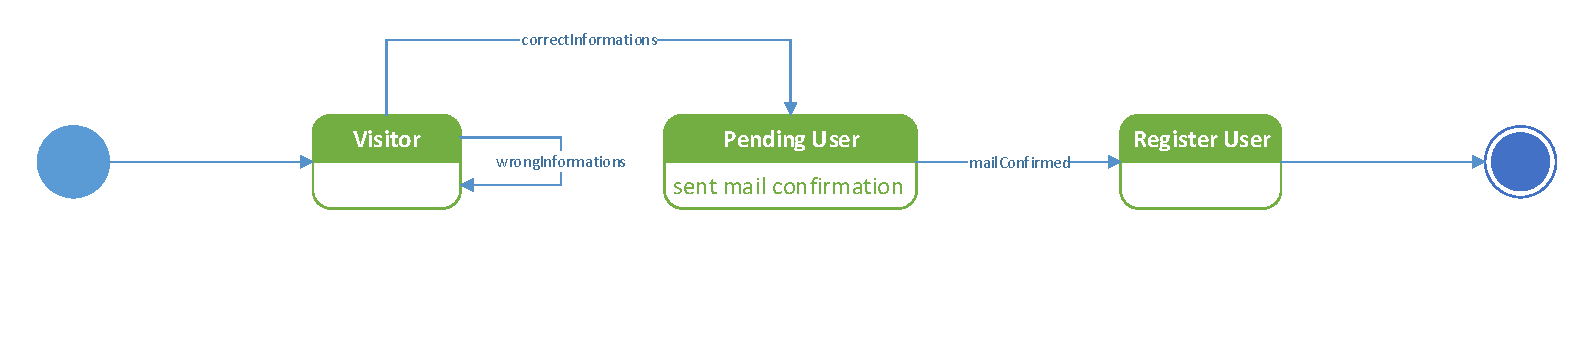
\includegraphics[width=\textwidth]{diagrams/registration_state}
	\end{center}

\paragraph{Functional Requirements}
	\begin{itemize}
		\item Visitors can register either as passengers or as taxi drivers.
		\item Visitors can abort the registration process at any time.
		\item The link in the confirmation email must be clicked within 1 day, otherwise the registration is deleted along with the visitor's info.
		\item Registration forms contain the following info (fields):
		\begin{itemize}
			\item email address
			\item username
			\item password
			\item password confirmation
			\item name
			\item surname
			\item (*) address
			\item (*) telephone number
			\item (**) taxi license ID
			\item (**) taxi plate number
			\item (**) taxi code
		\end{itemize}
		All fields must be contain valid inputs.\\
		Fields marked with (*) are not mandatory.\\
		Fields marked with (**) are only for taxi driver registrations.
		\item email address and username cannot be the same as ones from other myTaxiService users.
		\item password must contain at least 8 characters.
		\item password and password confirmation must match.
	\end{itemize}

\subsection{Login}
	\paragraph{Purpose}
		Visitors on myTaxiService website or mobile application may access to an existing registered user account providing its corresponding username (or email address) and password. In case the submitted info do not match with any existing account info, the system notifies the visitor that the username/email address doesn't exist, or that it exists, but the submitted password is wrong.\\
		In case a user forgets his/her password, the system allows him/her to retrieve it, automatically creating a new password, setting it as the user's one and sending it to the provided email address.

	\paragraph{Scenarios}
		\begin{enumerate}
			\item Carl is a passenger user. He opens myTaxiService website, but can't remember his password to access the service. Therefore, he clicks on "Forgotten password?". The system asks him for the email address or username he provided at registration. He writes it down and clicks "Confirm". The system verifies the existence of the submitted email address, then creates a new password and sends it in an email to the submitted email address.
			
			\item Daisy is a passenger user, familiar with the myTaxiService website. She wants to use the mobile app, too. Knowing that she can enter either username or email and password, she fills both fields and clicks on "Log in". The system verifies her info: the operation ends successfully, and she gains access to the passenger user homepage.
		\end{enumerate}

	\paragraph{Diagrams}
		\begin{center}
			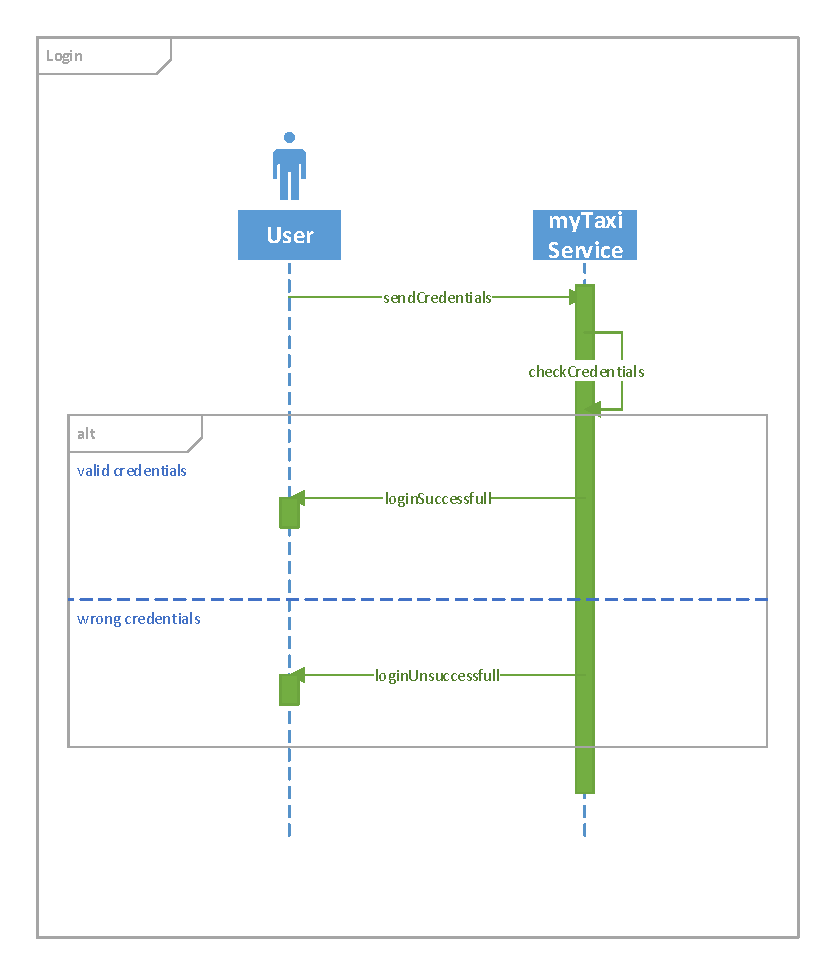
\includegraphics[height=\textwidth]{diagrams/login}
		\end{center}
		\begin{center}
			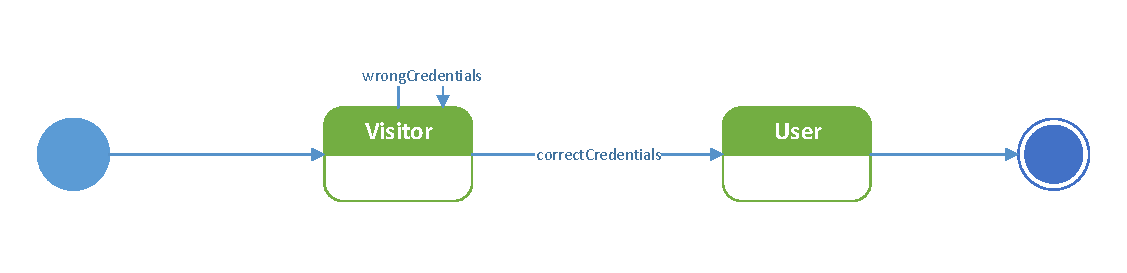
\includegraphics[width=\textwidth]{diagrams/login_state}
		\end{center}

	\paragraph{Functional Requirements}
		\begin{itemize}
			\item Visitors can log in either as passengers or as taxi drivers.
			\item Visitors must fill the "username" field either with an existing username or with an existing email address in order to successfully log in.
			\item Visitors must fill the "password" field with the only password corresponding to the submitted username/email address in order to successfully log in.
			\item The system will ignore log in requests if at least one of the "username" and "password" fields are left blank.
			\item The system allows visitors to retrieve their password if they forget it, by clicking "Forgot password?".
			\item The system requires visitors to submit an existing email address in the "username" field in order to retrieve their password.
			\item The system will take care of assigning the user a new password, when he/she states to have lost the previous one.
			\item The system will take care of sending to the email address submitted by the visitor the new assigned password, when he/she states to have lost the previous one.
			\item The system allows visitors to retrieve their password once a day.
		\end{itemize}
	
\subsection{Standard ride request}
	\paragraph{Purpose}
		Passenger users can request a taxi both through the web or through the mobile application, giving only simple data about the number of passengers and sharing preferences (in case of shared ride, see also 3.2.5, "Shared Ride Request").\\
		In any case, the system will then care about keeping the user informed about all details of his request, i.e. status of the request, estimated time of arrival (ETA) of the incoming taxi, in addition to its taxi code.
	
	\paragraph{Scenarios}
		\begin{enumerate}
			\item Elsa wanted to take the bus, but the heavy snow that fell in the last three days caused a lot of traffic problems. Fortunately for her, the taxi service is still functioning, so she opens myTaxiService on her mobile phone, logs in, and chooses "Request".
			She uses the GPS info to fill the "Origin" field, leaves the "Share" checkbox blank, then "Confirm". In a matter of minutes Frank, a taxi driver in her zone, accepts her request: Elsa is informed that she has to wait approximately 6 minutes for her taxi, encoded 288, to arrive. In the meanwhile, the system give her updates about the taxi position. At the expected time Frank arrives, picks Elsa up and carries her to desired destination.
		\end{enumerate}
	
	\paragraph{Diagrams}
		\begin{center}
	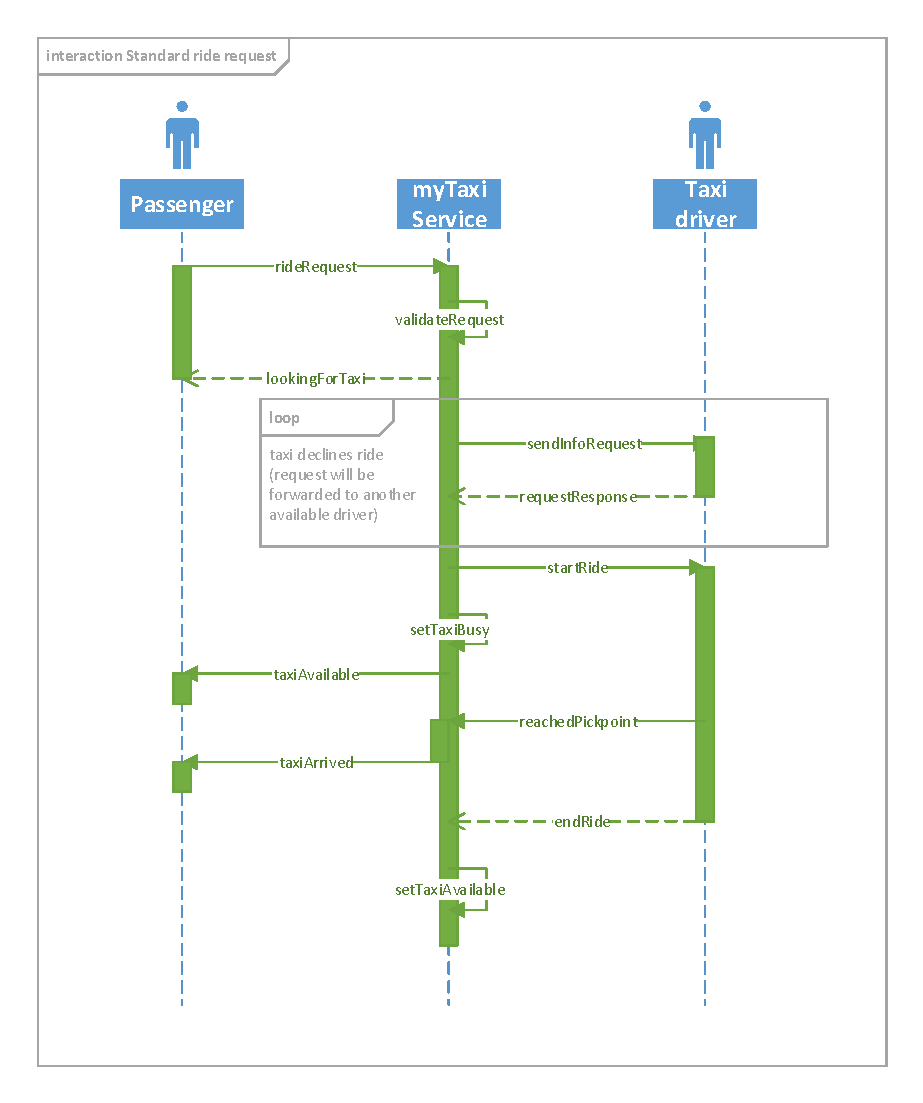
\includegraphics[width=\textwidth]{diagrams/standard_request}
\end{center}
\begin{center}
	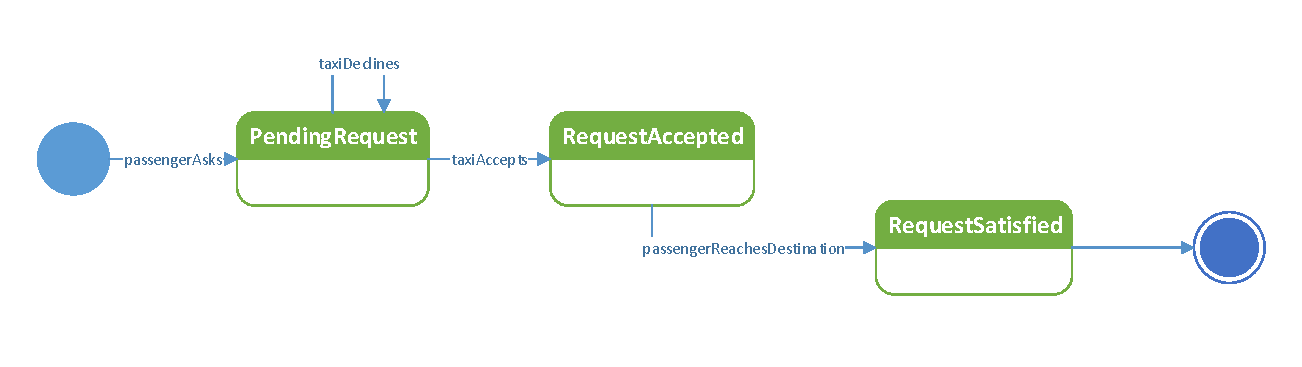
\includegraphics[width=\textwidth]{diagrams/standard_state}
\end{center}
	
	\paragraph{Functional Requirements}
		\begin{itemize}
			\item The system allows standard taxi ride requests to passenger users.
			\item The system allows standard taxi ride requests both on the web and on the mobile application.
			\item The system allows taxi ride requests if and only if the passenger accepts to give info about his/her location, either through GPS or directly writing down a valid location.
			\item The system allows taxi ride requests if and only if the passenger can be located in some definite position of some definite taxi zone.
			\item The system uses default values for the number of passengers and sharing preferences of a ride (1 person, no sharing), unless the passenger does specify them.
			\item The system uses a FIFO policy to manage forwarding of pending ride requests.
			\item The system uses a FIFO policy to manage the order of taxi drivers in queues to send notifications to.
			\item The system forwards a ride request to the first taxi driver in the considered zone queue if and only if he/she has a sufficient number of free seats available in his/her vehicle.
			\item The system keeps the passenger(s) notified about the status of the ride request he/she sent.
			\item Once a ride request has been accepted by some taxi driver, the system changes the request status from "Pending" to "Accepted".
			\item Once a ride request has been accepted by some taxi driver, the system calculates the ETA of the incoming taxi based on the distance between the taxi and the passenger(s), and the current traffic.
			\item Once a ride request has been accepted by some taxi driver, the system notifies the passenger(s) about the ETA of the incoming taxi.
			\item Once a ride request has been accepted by some taxi driver, the system keeps the passenger(s) notified about the current location of the incoming taxi, showing its position on a map.
			\item Once a ride request has been accepted by some taxi driver, the system prevents the passenger(s) to make a new ride request until the taxi driver changes the status of the ride to "Completed".
		\end{itemize}
		
\subsection{Reserved ride request}
	\paragraph{Purpose}
		Passenger users can request to reserve a taxi for some definite future ride. The operation can be done both through the web or through the mobile application, and requires information about the location and exact date and time of the meeting point, the destination, the number of passengers and the sharing preferences (in case of shared ride, see also 3.2.5, "Shared Ride Request").\\
		In any case, the system will take care about forwarding a taxi ride request to taxi drivers exactly 10 minutes before the agreed date and time. Reservation requests must occur at least two hours before the ride meeting time.
	
	\paragraph{Scenarios}
		\begin{enumerate}
			\item George has an important meeting tomorrow morning, but his car suddenly broke. He decides he will take a taxi. Therefore, he opens the homepage of myTaxiService web application on his laptop, logs in as a passenger user, then clicks "Reserve". He selects "use maps" for both position fields, and pinpoints his home and the location of the meeting as "Origin" and "Destination", respectively. He selects "7.15" as the meeting time, leaves the "Share" checkbox blank, then clicks "Confirm".\\
			The next day, at 7.05, a reserved ride requests is received by Harry, the first taxi driver in the queue of the taxi zone where George's meeting point is located. Harry decides to refuse the request, though. The request is then forwarded to Isabelle, which was the second taxi driver in queue at the time of Harry's refusal. She accepts George's request, and at the given time arrives at his house. She picks him up and brings him to the meeting.
		\end{enumerate}
	
	\paragraph{Diagrams}
		\begin{center}
	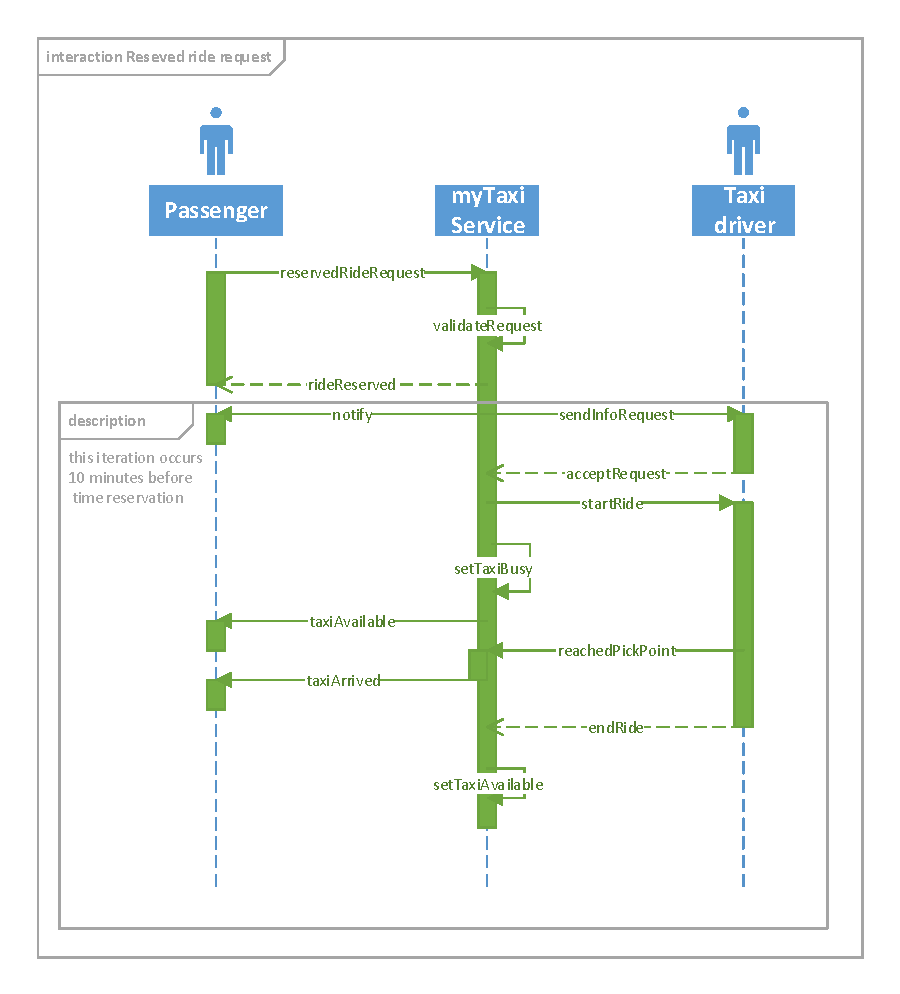
\includegraphics[width=\textwidth]{diagrams/reserved_request}
\end{center}
\begin{center}
	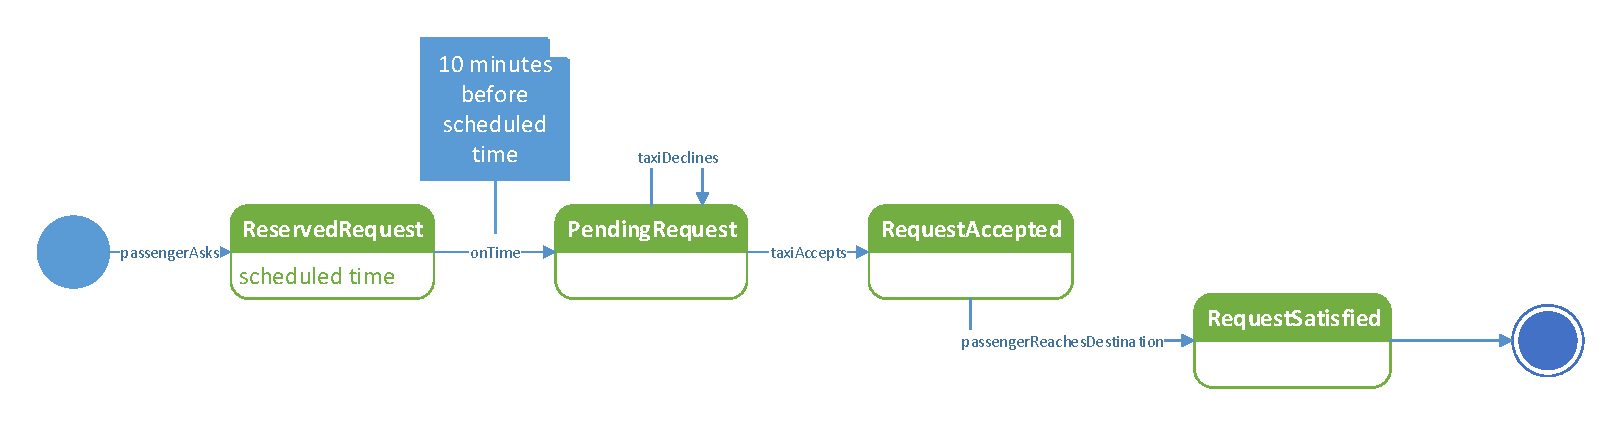
\includegraphics[width=\textwidth]{diagrams/reserved_state}
\end{center}

	\paragraph{Functional Requirements}
		\begin{itemize}
			\item The system allows reserved taxi ride requests to passenger users.
			\item The system allows reserved taxi ride requests both on the web and on the mobile application.
			\item The system allows reserved taxi ride requests if and only if the passenger gives definite existing positions of some definite existing taxi zones both for "Origin" and "Destination" fields.
			\item The system allows passengers to select locations either through GPS or directly writing down a valid location.
			\item The system allows reserved taxi ride requests if and only if the passenger gives complete info about the date and the time of the meeting.
			\item The system allows reserved taxi ride requests if and only if the time of the request occurs at least two hours before the ride meeting time.
			\item The system forwards notifications to taxi drivers about reserved taxi ride requests 10 minutes before the ride meeting time.
			\item The system uses default values for the number of passengers and sharing preferences of a reserved ride (1 person, no sharing), unless the passenger does specify them.
			\item The system uses a FIFO policy to manage forwarding of pending ride requests.
			\item The system uses a FIFO policy to manage the order of taxi drivers in queues to send notifications to.
			\item The system forwards a reserved ride request to the first taxi driver in the considered zone queue if and only if he/she has a sufficient number of free seats available in his/her vehicle.
			\item Once a reserved ride request has been accepted by some taxi driver, the system changes the request status from "Pending" to "Accepted".
			\item Once a reserved ride request has been accepted by some taxi driver, the system calculates the ETA of the incoming taxi based on the distance between the taxi and the passenger(s), and the current traffic.
			\item Once a reserved ride request has been accepted by some taxi driver, the system notifies the passenger(s) about the ETA of the incoming taxi.
			\item Once a reserved ride request has been accepted by some taxi driver, the system keeps the passenger(s) notified about the current location of the incoming taxi, showing its position on a map.
			\item Once a reserved ride request has been accepted by some taxi driver, the system prevents the passenger(s) to make a new ride request until the taxi driver changes the status of the ride to "Completed".
		\end{itemize}

\subsection{Shared ride request}
	\paragraph{Purpose}
		All ride requests can be shared with other passengers, in order to divide the cost of the ride. To do so, while subscribing a ride request, passenger users may specify their preference to share the ride, besides submitting a valid destination (if not already present).\\
		At the time of forwarding the request to taxi drivers, the system will use an appropriate algorythm to try to identify other ride requests with the same origin and a similar direction. The result will be an arrangement of those rides requests, taking into account the total number of seats necessary and calculating the optimal route to reach each destination in the least total time. The system will then proceed to forward the grouped requests as normal. In case a grouped request is not accepted, or continuously refused, for 3 minutes, the system proceeds to split the group and try to find new arrangements.\\
		When a grouped request is successfully accepted by some taxi driver, the system will take care of splitting the taxi fee among all passengers, proportionally to the distance traveled by each one.
	
	\paragraph{Scenarios}
		\begin{itemize}
			\item Jack and his friend Kevin want to go home after a party. They drank a bit too much, and Jack doesn't feel sober enough to drive. Therefore, he opens myTaxiService mobile application, logs in as a passenger user, and chooses "Request". Jack and Kevin don't have much money left, though, so Jack decides to share the ride. He ticks the "Share" checkbox, writes down his address as "Destination", then selects "Confirm". After a while Lara, who was at the same party and lives between Jack and her current position, sends a similar shared ride request, with destination her home. The system arrange the two requests in the same taxi. A minute after, Mark, a taxi driver, accepts the grouped request, and comes to pick up the three. He brings Lara home first, making her pay one third of the traveled distance. Then, Mark proceeds to Jack's home, and upon arrival makes Jack and Kevin pay the remaining cost of the ride. They decide to each pay half the fee.
			
			\item Neil has bought a ticket to the finals of his favourite team. Considering that during the day of the match it's almost impossible to find parking near the stadium, he decides go there by taxi. On his computer, he access the homepage of myTaxiService web application, logs in as a passenger user, then clicks "Reserve". He chooses an hour before the beginning of the match as Date and Time, ticks "Share" checkbox, selects his home as "Origin" and the stadium as "Destination" from the maps, then "Confirm". The system informs him that the request is successful. The system verifies the existence of other suitable shared ride requests to group Neil's one with, but doesn't find anything.\\
			The day of the match Oliver, another fan who lives in the same street of Neil, jumps to his same conclusion. A bit more than an hour before the match, he requests a shared ride from home to the stadium. Fortunately for him, no request was made that was eligible to be grouped with Neil's, so the system proceeds to group them. After a few minutes, Petra accepts Neil and Oliver grouped request, and comes to pick them up. Upon arrival, they split the ride fee equally.
		\end{itemize}
	
	\paragraph{Diagrams}
	\begin{center}
	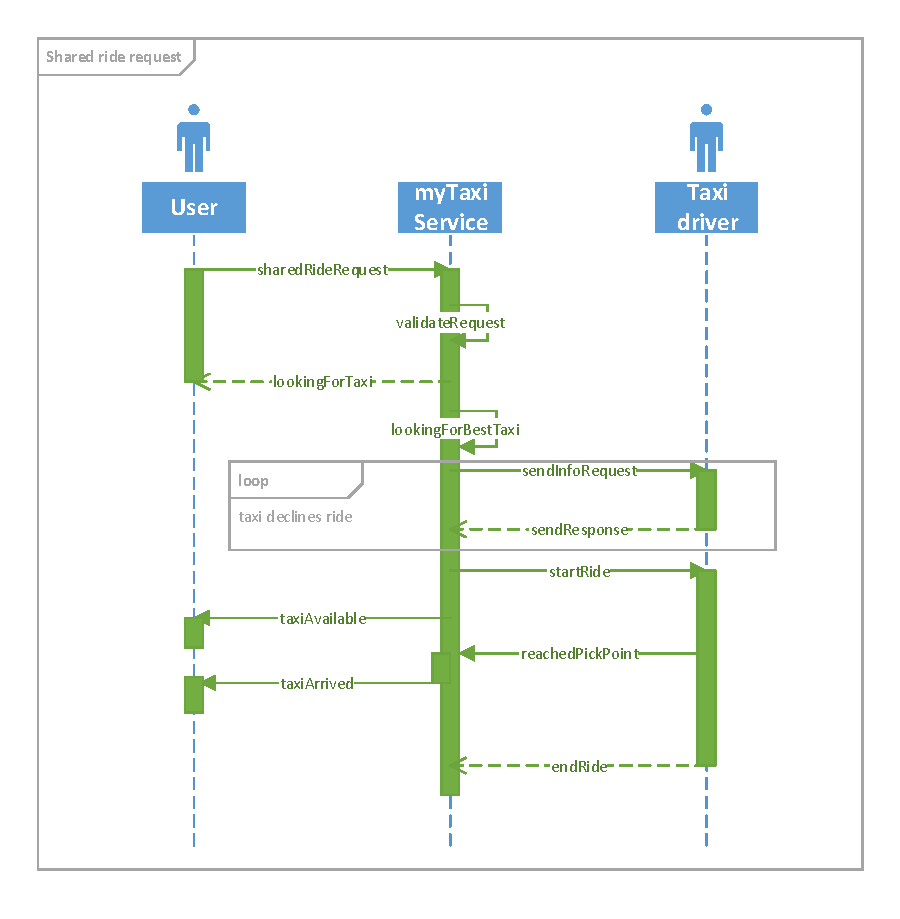
\includegraphics[width=\textwidth]{diagrams/shared_request}
\end{center}
\begin{center}
	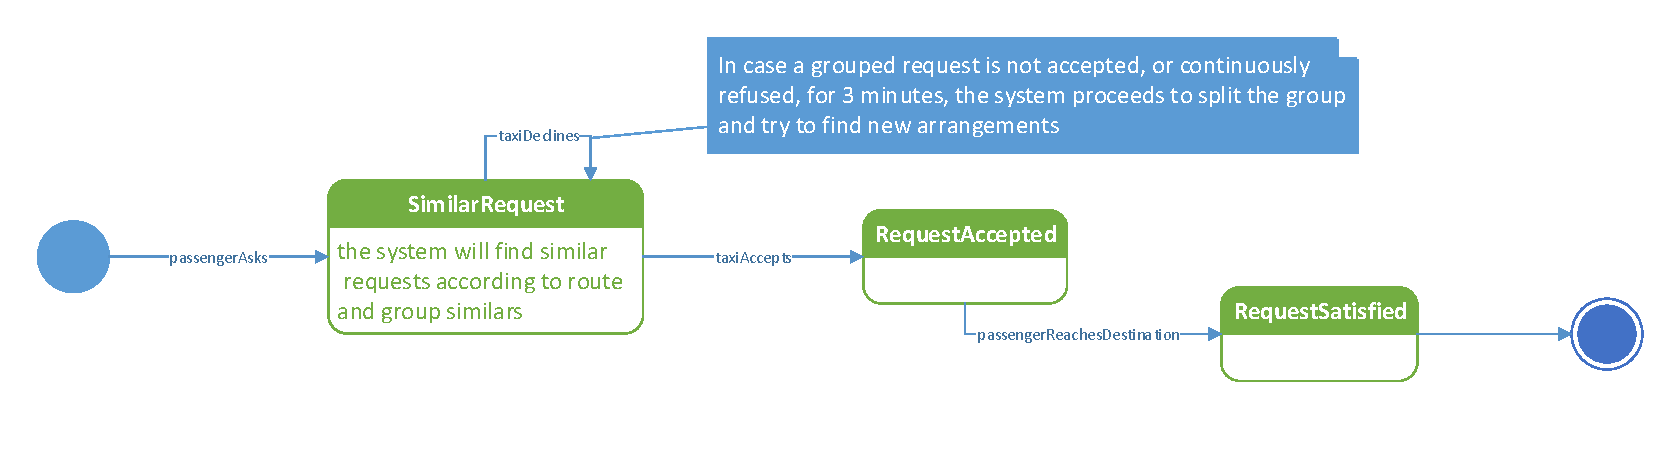
\includegraphics[width=\textwidth]{diagrams/shared_state}
\end{center}
	
	\paragraph{Functional Requirements}
		\begin{itemize}
			\item The system allows taxi ride sharing to passenger users.
			\item The system allows taxi ride sharing both on the web and on the mobile application.
			\item The system allows both standard shared taxi ride requests and reserved shared taxi ride requests, simply ticking the "Share" checkbox while doing any any kind of taxi ride request.
			\item Both kinds of shared ride requests require no less data than their non-shared forms (see also 3.2.3, "Standard ride request" and 3.2.4, "Reserved ride request").
			\item The system allows standard shared taxi ride requests if and only if the passenger also gives a definite existing position of some definite existing taxi zone as "Destination" (reserved taxi ride requests already require this, even if non-shared).
			\item The system allows passengers to select the input for "Destination" either through GPS or directly writing down a valid location.
			\item The system, at the time of forwarding any shared ride request, will use a special algorythm to calculate good arrangements between different shared ride requests.
			\item The arrangement algorythm search different shared ride requests to form a single, grouped, shared ride request.
			\item The arrangement algorythm considers for grouping only shared rides with close "Origin" positions and similar directions towards "Destination" positions. Similar directions means that going from the origin to the farthest destination implies passing by the other destination(s) as well.
			\item The arrangement algorythm also considers the total number of passengers in a taxi. Groups that would occupy too many seats are not eligible.
			\item The arrangement algorythm can group even standard and reserved ride requests together, as long as all the others requirements are met.
			\item The system will consider group requests as a single one when forwarding them to taxi drivers.
			\item Taxi drivers can see all details of all shared requests when receiving notification of a grouped request.
			\item Taxi drivers can accept or refuse grouped requests as normal.
			\item The system will automatically split up groups of shared requests if they're continuously refused, or simply not accepted, for 3 minutes since their forwarding.
			\item The system will then proceed to recalculate possible groups with the special algorythm, but excluding the arrangements that were already tried.
			\item The system calculates how to split taxi fees equally on all passengers on a shared ride, depending on the distance traveled by each one and the number of passengers during each part of the ride.
			\item The system notifies the taxi driver how much of the total fee each passenger will have to pay, in percentage.
		\end{itemize}
	
\subsection{Request notification and response}
	\paragraph{Purpose}
		Taxi driver users, if logged in on the myTaxiService mobile application and not busy, are able to receive notifications about pending ride requests. They then become able to respond to them, either accepting or refusing.\\
		The system manages taxis assigning each taxi driver to the queue of his/her corresponding taxi zone. Every request notification from a certain zone is forwarded to the first eligible taxi driver of that taxi zone queue. If that first taxi driver accepts it, the request becomes accepted and the taxi driver status changes to "Busy": he/she is removed from the queue. He/she will be put back on the bottom of the queue as soon as he notifies the system that he's finished the ride and his/her status changes back to "Ready".\\
		If the first taxi driver refuses instead, the request is forwarded to the second taxi driver; the same goes for the third, the fourth and so on. Either way, taxi drivers that refuse a request end on the bottom of their taxi zone queue. Finally, taxi drivers must respond to each request within one minute from its forwarding, otherwise the system will automatically take it as a refusal.
	
\paragraph{Scenarios}
		\begin{itemize}
			\item Pamela is a taxi driver. She's a few minutes from ending her workshift before launchbreak, when suddenly a new request notification arrives on the myTaxiService application on her mobile phone. The request comes from passenger user Qasim. Pamela can see his position on the map. He's pretty far from her current position, so she decides to refuse and end her workshift. The system changes her status to "Offline".\\
			Qasim's request is instead forwarded to the next taxi driver user in the same zone queue, Rebecca. She decides to accept the request, thus changing her status from "Ready" to "Busy" and leaving the taxi zone queue. Qasim is notified that his request has been accepted. Rebecca goes to pick him up and brings him to his destination.
			
			\item Simon is a taxi driver user. It's late in the night and he's really tired: without noticing, he dozes off. Not long after, a notification arrives on his mobile phone. It's a shared request from passenger users Thomas and Ursula. Unfortunately, Simon doesn't notice it: one minute passes and the system automatically take it as a refusal. The grouped request is forwarded to taxi driver Violet, who decides to accept it: the system removes her from the queue and changes her status to "Busy". Thomas and Ursula are both notified that they're request have successfully been accepted, and that Violet is on her way to them. Some minutes after, Violet arrives and bring them to their destination, splitting the fee according to the system indications.
		\end{itemize}
		
	\paragraph{Diagrams}
	\begin{center}
	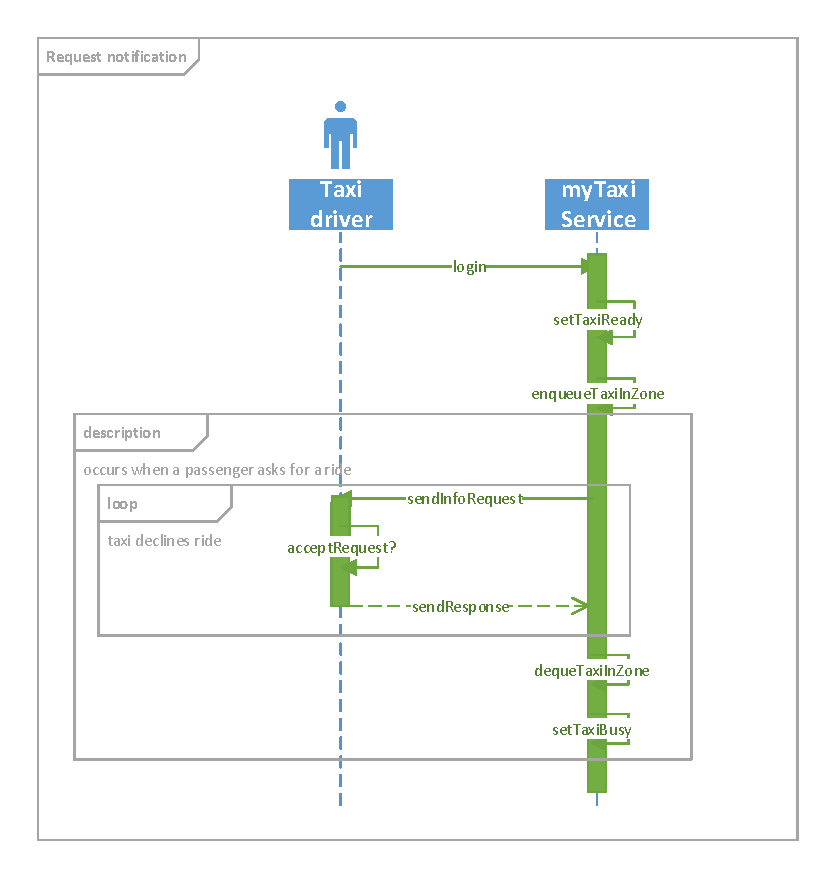
\includegraphics[width=\textwidth]{diagrams/notification}
\end{center}
\begin{center}
	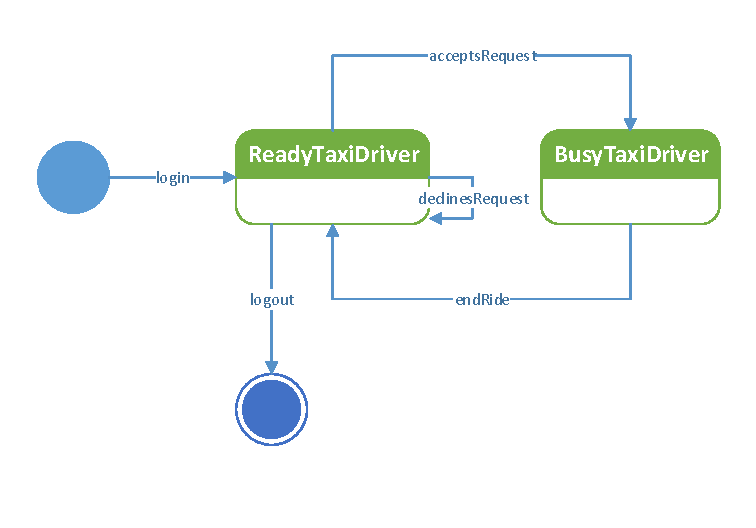
\includegraphics[width=\textwidth]{diagrams/request_state}
\end{center}
	
	\paragraph{Functional Requirements}
		\begin{itemize}
			\item The system allows taxi drivers to receive ride request notifications on their mobile phone application and respond to them, either accepting or refusing.
			\item The system notifies taxi drivers about all request notifications forwarded to them.
			\item The system uses a FIFO policy to manage forwarding of pending ride requests.
			\item The system uses a FIFO policy to manage the order of taxi drivers in queues to send notifications to.
			\item The system forwards a ride request to the first taxi driver in the considered zone queue if and only if he/she has a sufficient number of free seats available in his/her vehicle.
			\item Taxi zone queues contain only taxi drivers that currently have status "Ready".
			\item Taxi zone queues contain only taxi drivers that are currently located in that taxi zone.
			\item Taxi ride notifications show all requesting passengers' username and position on a map.
			\item The system gives taxi drivers one minute to accept or refuse request notifications, otherwise take it as a refusal. This is to avoid long waiting times for passengers.
			\item Once a ride request has been accepted by some taxi driver, the system changes his/her status to "Busy" and he/she's removed from his/her taxi zone queue.
			\item The system allows taxi drivers to notify the end of the ride, when they're doing one (i.e. when they accepted a ride request).
			\item Once a taxi driver notifies the end of a ride, the system changes his/her status to "Ready" and he/she's put on the bottom of his/her taxi zone queue.
		\end{itemize}

\subsection{Availability settings}
	\paragraph{Purpose}
		Taxi drivers are able to notify the system about their status through the mobile application at any moment, as long as they're logged in. In particular, the status can be either "Ready", "Busy" or "Offline".\\
		Whenever a taxi driver logs in, the system automatically sets his/her status from "Offline" to "Ready" and put him/her on the bottom of its current taxi zone queue, based on GPS info.\\
		When he/she accepts a taxi ride, the status is automatically updated to "Busy": the system then removes him/her from the queue, preventing the arrival of other ride requests.\\
		Similarly, when the ride is over, the taxi driver has to notify the system that the ride has ended: the system automatically changes the status back to "Ready" and puts him/her back on the bottom of the current taxi zone queue, thus waiting for a new ride request.\\
		Finally, when the taxi driver finishes his workshift, he may inform the system, or simply log off. In both cases, his/her status automatically switches to "Offline".

	\paragraph{Scenarios}
		\begin{itemize}
			\item William is a taxi driver subscribed to myTaxiService. He logs in through his mobile phone and his status changes from "Offline" to "Ready". The system receives info from the GPS and puts William on the bottom of the taxi zone he's currently in. After a while, his phone notifies him about a new ride request: it's from passenger user Xenia. William decides to accept it and his status changes to "Busy". He's no longer in the taxi queue. William goes to the start location, picks up Xenia and takes her to her destination. When they arrive, William informs the system that he has concluded the ride: his status changes to "Ready". The system puts him on the bottom of his current taxi zone queue. Later on, he receives another ride requests, but this time he decides to refuse it: its status remains unchanged as "Ready", but he loses all his positions in the queue. A few hours later, William finishes his worktime and logs off. The system sets his status to "Offline" and removes him from any queue.
		\end{itemize}
	
	\paragraph{Diagrams}
		\begin{center}
			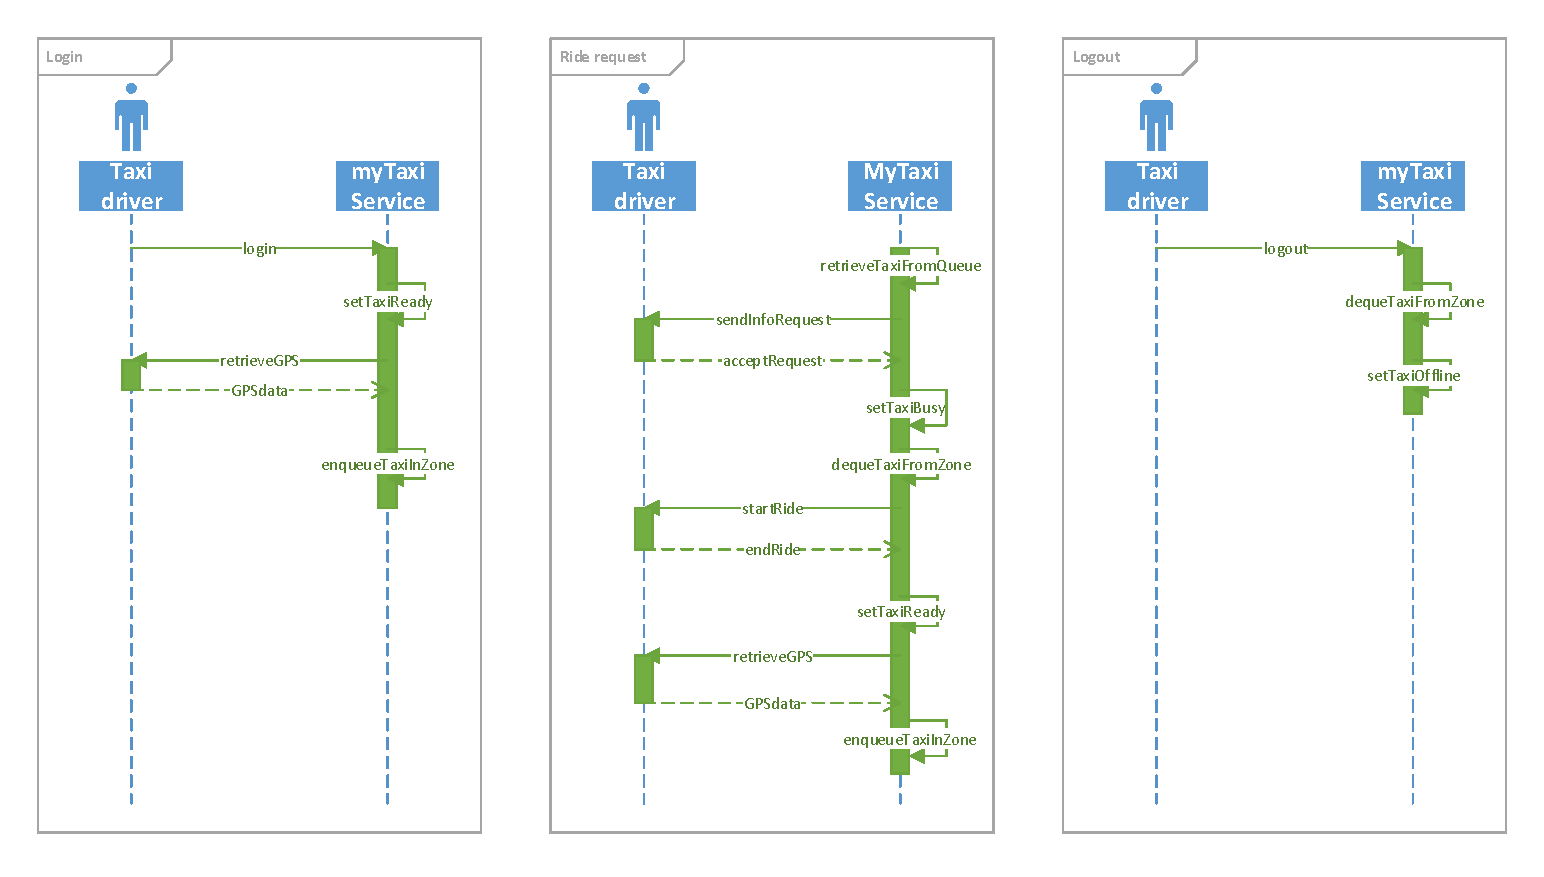
\includegraphics[width=\textwidth]{diagrams/availability}
		\end{center}
		\begin{center}
			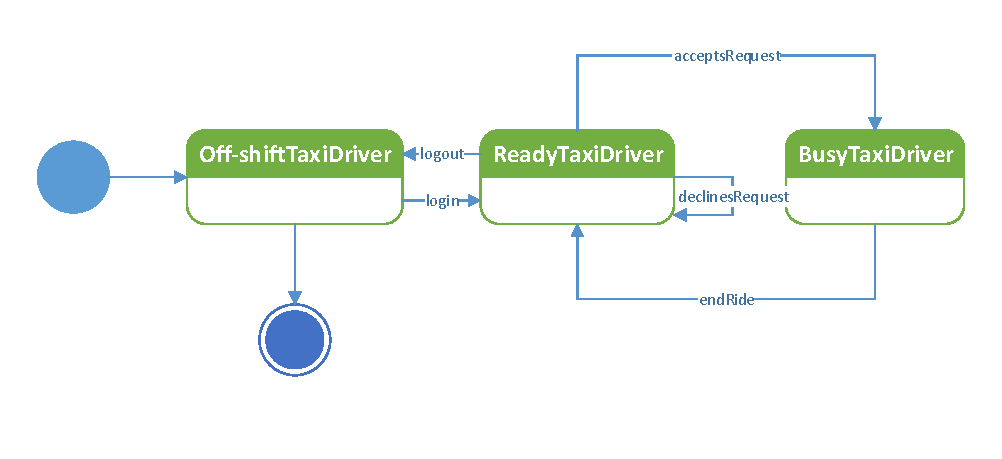
\includegraphics[width=\textwidth]{diagrams/availability_state}
		\end{center}
		
	\paragraph{Functional Requirements}
		\begin{itemize}
			\item The system uses a FIFO policy to manage taxi zone queues.
			\item The system uses info provided by the GPS to locate taxis and decide their respective queues.
			\item The system automatically inserts taxi drivers in queues when their status changes to "Ready".
			\item The system automatically removes taxi drivers from queues when their status changes to "Busy" or "Offline".
			\item The status automatically changes to "Busy" when the taxi driver accepts a ride request.
			\item The status automatically changes to "Ready" when the taxi driver notifies the end of a ride.
			\item When status is "Ready", the application notifies about ride requests.
			\item When status is "Ready", the application enables the taxi driver to accept/refuse requests.
			\item When status is "Busy", the application prevents ride requests notifications.
			\item When status is "Busy", the application enables the taxi driver to notify the end of the current ride.
		\end{itemize}

\subsection{Account settings}
	\paragraph{Purpose}
		The system allows registered users to view and modify their profiles at any moment, as long as they're logged in. Usernames cannot be modified, while modified email addresses, taxi license IDs and taxi codes must not match with the ones of other users, otherwise the system denies the modification request. In case of modified email address, the system sends a confirmation email to the new address. Modification will successfully ends when the user clicks the link in the sent email.
	
	\paragraph{Scenarios}
		\begin{itemize}
			\item Zac uses to periodically change his account password, in order to increase protection. To do so, every 3 months, he opens myTaxiService on his mobile phone, chooses "Profile", then "Modify". He selects the password field, writes down a new one, then writes it again in the "Confirm password" field. Finally, he clicks "Confirm": the system informs him that his account password has successfully been updated.
		\end{itemize}
	
	\paragraph{Diagrams}
		\begin{center}
			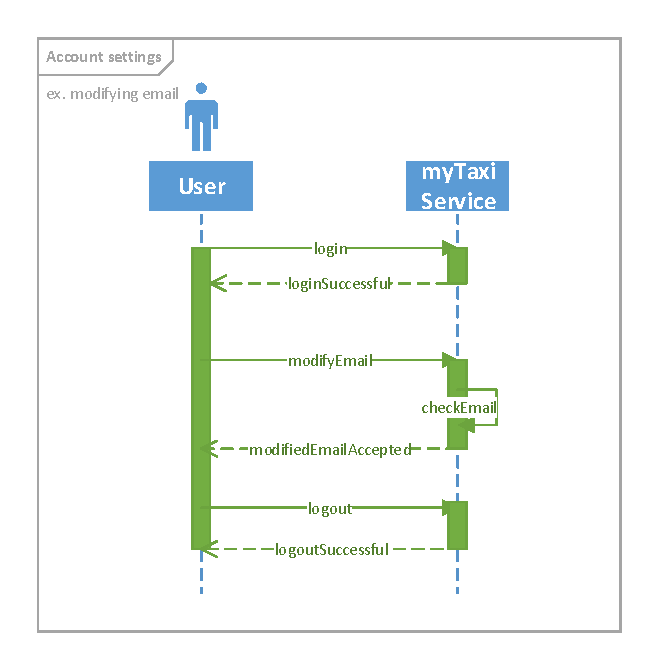
\includegraphics[width=\textwidth]{diagrams/account_settings}
		\end{center}
			\begin{center}
				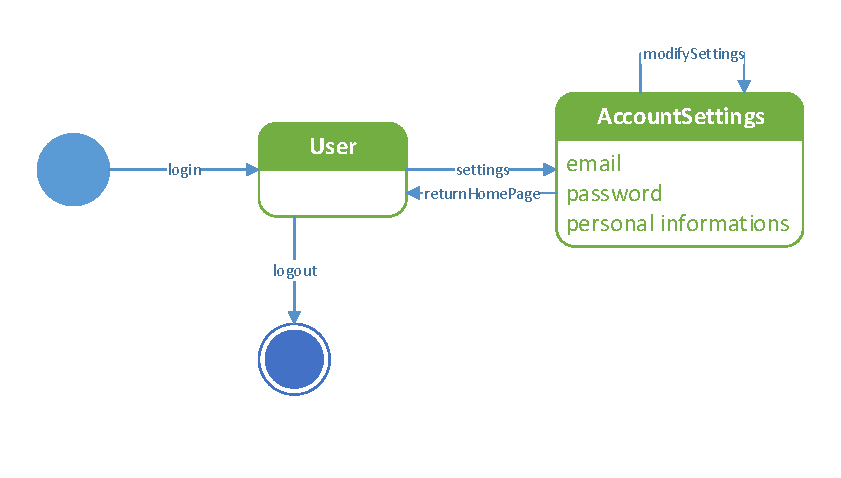
\includegraphics[width=\textwidth]{diagrams/settings}
			\end{center}
	
	\paragraph{Functional Requirements}
		\begin{itemize}
			\item Account settings are available to both passenger and taxi driver users.
			\item Account settings are available both on the web and the mobile application.
			\item Account settings are accessible from the start screen of both apps, through the "Profile" button.
			\item The system allows users to view all their profile info, submitted during registration (see also 3.2.1, "Registration").
			\item The system allows users to modify all their profile info, submitted during registration, with the only exception of username.
			\item Modifying the password requires to write the old one, and the new one twice; if the former password is not correct or if the two new passwords submitted do not match, the system asks for all passwords again and notifies the user.
			\item Modifying the email address, the taxi license ID or the taxi code requires that the new one doesn't match with the one of another registered user.
			\item Modifying the email address requires confirmation through an email sent to the submitted email address.
			\item The system allows users to abort modifications at any time.
			\item The system allows users to delete their account: confirmation is required to proceed.
		\end{itemize}
